%%%%%%%%%%%%%%%%%%%%%%%%%%%%%%%%%%%%%%%%%%%%%%%%%%%%%%%%%%%%%%%%%%%%%%%%%%%%%%%%%%%%%%%%%%%%%%%%%%%%%%%%%%%%%%%%%%%%%%%%%%%%%%%%%%%%%EJERCICIO 9 %%%%%%%%%%%%%%%%%%%%%%%%%%%
    \textbf{Ejemplo 9}\\
	Amortizar en valor constante la suma de 500.000 COP mediante 3 pagos anuales que decrecen en 20.000 COP; suponga un interés del 10\% periódico anual vencido  y una tasa única de corrección monetaria del 24\% nominal anual año vencido.\\			
				
	\textbf{Solución 9}\\
	%La tabla ira centrada
	\begin{center}
		\renewcommand{\arraystretch}{1.5}% Margenes de las celdas
		%Creación de la cuadricula de 3 columnas
		\begin{longtable}[H]{|p{0.5\linewidth}|p{0.5\linewidth}|}
			%Creamos una linea horizontal
			\hline
			%Definimos el color de la primera fila
			\rowcolor[HTML]{FFB183}
			%%%%% INICIO ASIGNACIÓN período FOCAL %%%%%%%
			%%%%%%%%%% INICIO TITULO
			%Lo que se hace aquí es mezclar las 3 columnas en una sola
			\multicolumn{2}{|c|}{\cellcolor[HTML]{FFB183}\textbf{1. Asignación período focal}}   \\ \hline
			%%%%%%%%%% FIN TITULO
			%%%%% INICIO DECLARACIÓN DE VARIABLES %%%%%%%
			\multicolumn{2}{|c|}{$pf = 0 \textit{ pav}$}\\ \hline
			%%%%%%%%%% INICIO TITULO
			%Lo que se hace aquí es mezclar las 3 columnas en una sola
			\multicolumn{2}{|c|}{\cellcolor[HTML]{FFB183}\textbf{2. Declaración de variables}}   \\ \hline
			%%%%%%%%%% FIN TITULO
			%%%%%%%%%% INICIO DE MATEMÁTICAS
			%Cada & hace referencia al paso de la siguiente columna
			$VP = 500.000 \ COP $  				& $R_{1} = ? COP    $  \\
			$i = 10\%  \hspace{1mm} pav$      	& $R_{2} = ? COP    $ \\
			$ n = 3 \hspace{1mm} pav $          & $R_{3} = ? COP    $ \\ \hline
			%%%%%%%%%% FIN DE MATEMÁTICAS
			%%%%% FIN DECLARACIÓN DE VARIABLES
			
			\rowcolor[HTML]{FFB183}
			\multicolumn{2}{|c|}{\cellcolor[HTML]{FFB183}\textbf{3. Diagrama de flujo de caja}} \\ \hline
			\multicolumn{2}{|c|}{ 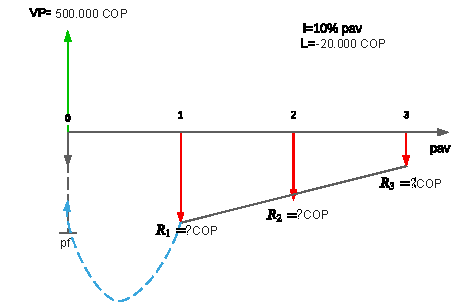
\includegraphics[trim=-78 -5 -78 -5]{7_Capitulo/img/ejemplos/9/9_1.pdf} }   \\ \hline
			%%%%% INICIO FLUJO DE CAJA
			\rowcolor[HTML]{FFB183}
			\multicolumn{2}{|c|}{\cellcolor[HTML]{FFB183}\textbf{4. Declaración de fórmulas}} \\ \hline
			%%%%%%%%%%%%% FIN INSERCIÓN DE IMAGEN
			%%%%%FIN FLUJO DE CAJA
			
			\multicolumn{2}{|c|}{ $VP = R\frac{1- (1+i)^{-n} }{i} + \frac{L}{i} ( \frac{1- (1+i)^{-n} }{i} - n(1+i)^{-n}) $ valor presente serie uniforme anticipada}   \\  \hline
			
			%%%%%% INICIO DESARROLLO MATEMÁTICO
			\rowcolor[HTML]{FFB183}
			%%%%%%%%%%INICIO TITULO
			\multicolumn{2}{|c|}{\cellcolor[HTML]{FFB183}\textbf{5. Desarrollo matemático}}       \\ \hline
			%%%%%%%%%% FIN TITULO
			%%%%%%%%%% INICIO MATEMÁTICAS
			\multicolumn{2}{|c|}{ $ 500.000 \ COP = R\frac{1- (1+i)^{-n} }{i} + \frac{L}{i} ( \frac{1- (1+i)^{-n} }{i} - n(1+i)^{-n}) $}   \\ 
			\multicolumn{2}{|c|}{ $ 500.000 \ COP = R\frac{1- (1+0,10)^{-3} }{0,10} + \frac{-20.000}{0,10} ( \frac{1- (1+0,10)^{-3} }{0,10} - 3(1+0,10)^{-3}) $}   \\ 
			\multicolumn{2}{|c|}{ $  R = 219.788,52  \ COP $}   \\ 
			\multicolumn{2}{|c|}{ $  R_{1} = 219.788,52 \ COP (1 + 0,24)^{1} =  272.537,76 \ COP $}   \\ 
			\multicolumn{2}{|c|}{ $  R_{2} = 199.788,52 \ COP (1 + 0,24)^{2} = 307.194,83 \ COP  $}   \\ 
			\multicolumn{2}{|c|}{ $  R_{3} = 179.788,52 \ COP (1 + 0,24)^{3} =   342.789,12 \ COP $}   \\  \hline
	
			%%%%%%%%%% FIN MATEMÁTICAS
			%%%%%% FIN DESARROLLO MATEMÁTICO
			%%%%%% INICIO RESPUESTA
			\rowcolor[HTML]{FFB183}
			%%%%%%%%%%INICIO TITULO
			\multicolumn{2}{|c|}{\cellcolor[HTML]{FFB183}\textbf{6. Respuesta}}   \\ \hline
			%%%%%%%%%% FIN TITULO
			%%%%%%%%%% INICIO RESPUESTA MATEMÁTICA
			\multicolumn{2}{|c|}{ 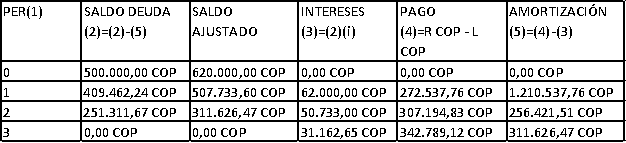
\includegraphics[trim=-78 -5 -78 -5]{7_Capitulo/img/ejemplos/9/9_2.pdf} }   \\ \hline
			%\multicolumn{2}{|C{\textwidth}|}{
			%	$R_{58} =72.478,16 \ COP (1 + 0,02)^{57} = 224.087,15 \ COP $ 
			%}  \\ \hline
			
			
			%%%%%%%%%% FIN MATEMÁTICAS
			%%%%%% FIN RESPUESTA
		\end{longtable}
		%Se crean dos lineas en blanco para que no quede el siguiente texto tan pegado
		%\newline \newline %USARLO SI CREES QUE ES NECESARIO
	\end{center}
 %%%%%%%%%%%%%%%%%%%%%%%%%%FIN EJERCICIO 9 %%%%%%%%%%%%%%%%%%%%%%%%%%%